\chapter{Felhasználói dokumentáció}
\label{ch:user}
\todo[inline]{Rövid bevezető a verziókezelésről.}
\section{A téradatok verziókezelésének problémája}
Téradatokkal -- vagy bármilyen kép alapú adatokkal -- egyre több szakterület dolgozik, és általánosan ezek a folyamatok kifejezetten magas számú felhasználók által végzett módosítással járnak. Az információk tárolása vagy binárisan, vagy valamilyen összetett geodéziai adatbázis állománnyal történik, ezek verziókövetésére pedig nem született még általánosan alkalmazható megoldás. A QGIS egy széles körben elterjedt, főleg térképészeti adatok létrehozását, módosítását és tárolását támogató szoftver, ami még nem rendelkezik verziókezelést megvalósító kiegészítéssel, a Q-Aegis modul ezen hiány betöltésére született.
\section{A modul működése}
A Q-Aegis plugin az AEGIS nevű téradatkezelő keretrendszer felhasználásával biztosítja a QGIS-ben létrehozott projektek műveletalapú verziókezelését. A verziókezelő és a szerkesztőprogram közti technikai különbségeket a nyílt forráskódú \emph{Python.Net} \cite{pythonnet} modul használatával hidalja át. A program követi a rétegek és a rajtuk lévő objektumok (\emph{feature}ök) változásait, a geometriák alakulását reverzibilis transzformációkká alakítja és ezeket tárolja. A korábbi vagy újabb verziók betöltésekor így nem szükséges forrásfájlokat cserélni, a rétegek új állapotait beállítani, mindez automatikusan megtörténik. Ezen kívül a megvalósítása miatt a Q-Aegis plugin lehetővé teszi, hogy a QGIS-ben végzett munka során csupán az eredetileg nem menthető memóriában tárolt rétegekkel dolgozzon a felhasználó.

\section{A beépülő modul telepítése}
\subsection{Rendszerkövetelmények}
Mivel a program egy beépülő modul (\emph{plugin}) a QGIS térinformatikai programhoz, ezért használatához szükséges legalább a szoftver 3.6-os verzió jelenléte. \todo{Szerintem írható az, hogy a 3.x verzió támogatott, tesztelve a 3.6-os verzióval lett.} Korábbi verziók esetén nem ismert viselkedések léphetnek fel, viszont a beépülő potenciálisan használható korábbi 3.x-es verziókkal is (nem tesztelt). Az AEGIS csomag használata miatt, amennyiben nincs még jelen a rendszerben, telepíteni kell a Microsoft .NET keretrendszert a legfrissebb verzióig \todo{Konkrétan .NET 4.0-ra épül a projekt, így az vagy újabb frissebb változat kell. Ez Windows alatt amúgy már az OS része.}. Az előbbi dependencia miatt a program csak Microsoft Windows operációs rendszer alatt használható. \todo{Bár végül nem a .NET Core változat lett felhasználva, de Mono révén így is használható Linux és MacOS alatt is.}
\subsection{Telepítés}
A beépülő telepítése kifejezetten egyszerű, csak ki kell csomagolni a mellékelt tömörített állomány tartalmát a helyi QGIS verzió \texttt{python/plugins} könyvtárába, amely telepítési könyvtár a \texttt{apps/qgis/python/plugins} útvonalán érhető el. Ezután a QGIS-t elindítva a \emph{Plugins / Manage and install plugins} menüponton keresztül megnyitott plugin kezelőben be kell kapcsolni a Q-Aegis plugint, hogy az ábrán látható állapotot kapjuk :
\begin{figure}[H]
	\centering
	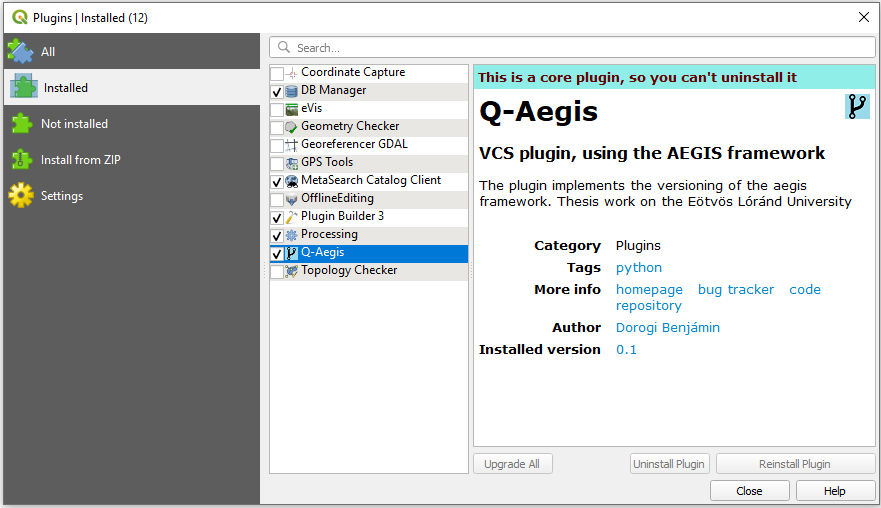
\includegraphics[width=\textwidth,height=250px]{images/enable_plugin}
	\caption{Az aktiválás utáni állapot}
	\label{fig:picture-1}
\end{figure}

Ezután a verziókezelő modul használatra kész.
	
\section{A verziókezelő használata}
\subsection{A kezelőfelület}
A beépülő modul a QGIS-en belül létrehozott projektekkel van összekötve, így amíg nem nyitunk meg egy projektet, nem érjük el az új funkciókat. Projekt megnyitása után \todo{Új projekt létrehozásakor is jó lenne ezt támogatni.} a modul kezelőfelülete a QGIS beépülő modulok eszköztárán található ikonra (\ref{fig:picture-2}.~ábra) kattintva nyitható meg, és a \ref{fig:picture-3}.~ábrán \todo{A $\sim$ a nem tördelt szóköz.} látható módon néz ki alapértelmezett állapotban.
\begin{figure}[H]
	\centering
	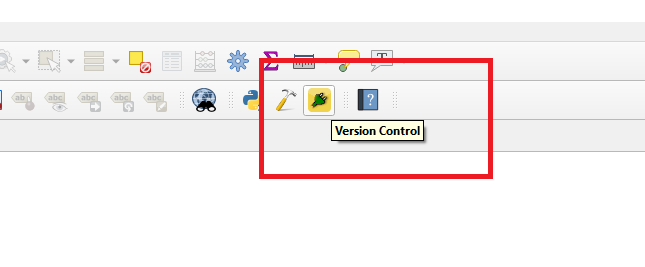
\includegraphics[width=0.8\textwidth,height=190px]{images/plugin_button.png}
	\caption{Az eszköztáron található ikon}
	\label{fig:picture-2}
\end{figure}
\begin{figure}[H]
	\centering
	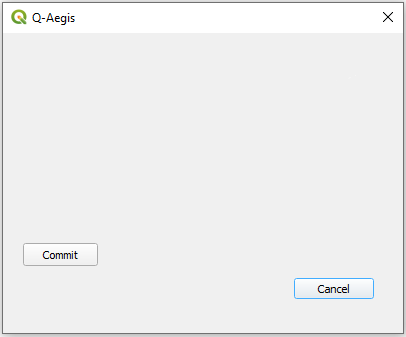
\includegraphics[width=0.8\textwidth,height=250px]{images/norepo_state.png}
	\caption{A kezelőfelület alapállapota}
	\label{fig:picture-3}
\end{figure}
Az ablak a \emph{Cancel} bezárás gombbal zárható be, a többi gomb funkciójára, valamint a felület esetleges változásaira a használatot magyarázó részekben térünk ki.
\subsection{Új követett projekt létrehozása}
Amennyiben teljesen üres projekttel szeretnénk elkezdeni a munkát, technikai okokból a projektet létre kel hozni, elmenteni, majd újra megnyitni. Ekkor létrejön a projekthez tartozó tároló, a verziókezelés használható innentől. \todo{Ez így nagyon körülményes, jobb lenne megnézni nem támogatható-e új projekt létrehozásakor is a verziókezelés.}
Ha már meglévő projektet szeretnénk verziókezelés alá vonni, akkor a projektfájl megnyitása után a kezelőfelületen található \emph{Commit} beküldés gombra kattintva a projekt teljes állapota bekerül a rendszerbe és a további módosítások már követhetőek lesznek.

\subsection{Módosítások mentése a verziókezelőbe}
Miután módosításokat végeztünk a projekten, a \emph{Commit} \todo{Angol szavakat érdemes tipográfiailag kiemelni, pl. dőlten szedni.} gomb újbóli megnyomásával az új állapot bekerül a revíziókezelő rendszerbe. A QGIS szerkesztési funkciói azok széles terjedelme miatt (egyelőre) nem teljes körűen támogatottak Q-Aegisben, hanem a következő alapvető módosítások kezeltek:
\begin{itemize}
	\item Új réteg hozzáadása
	\item Létező réteg eltávolítása
	\item Geometria hozzáadása réteghez
	\item Geometria eltávolítása rétegről
	\item Geometria módosítása:
	\begin{itemize}
		\item Tetszőleges geometria részének vagy egészének eltolása
		\item Vonal típusú geometriákba új pont felvétele, pontok eltávolítása vonalakból
		\item Poligon típusú geometriákhoz "lyukak" hozzáadása vagy eltávolítása
		\item Multigeometriákhoz részek hozzáadása vagy eltávolítása
	\end{itemize}	
\end{itemize}

\subsection{Tetszőleges verzió betöltése}
Amennyiben már van a projekthez mentett verzió, a kezelőfelület némileg megváltozik, megjelenik rajta egy lista az elérhető verziókról (~\ref{fig:picture-4}). A listából egy tetszőleges számú verziót kiválasztva, majd a "Load Version" gombra kattintva a projektbe betöltődik a kiválasztott verzió. Amennyiben a betöltés előtt a projektben vannak olyan módosítások, amelyek még nem kerültek be a rendszerbe, a program egy felugró ablakkal figyelmezteti a felhasználót, és felajánlja neki a lehetőséget, hogy commitolja a módosításait, mielőtt betöltené az új verziót.

Ha korábbi állapot van betöltve, és módosításokat végzünk rajta, akkor ha menteni próbálunk, a rendszer hibaüzenettel jelzi, hogy előbb a legfrissebb verzióra kell állni és utána lehet módosítani.
\begin{figure}[H]
	\centering
	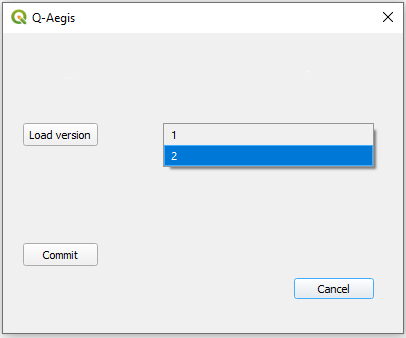
\includegraphics[width=0.8\textwidth,height=250px]{images/available_versions.png}
	\caption{A verzióválasztó lista}
	\label{fig:picture-4}
\end{figure}
\todo[inline]{Az ablak tartalmát kicsit rendezd. Ne legyenek fölöslegesen nagy térközök, a Commit és a Cancel gomb lehetne egy vonalban, ilyenek.}

\begin{note}
A QGIS több opcióval is rendelkezik arra, hogy milyen módon tároljuk a rétegeinket. A Q-Aegis csak a vektoros rétegtípusokon végzett műveleteket támogatja. Szerkesztés közben nem számít, hogy memóriában tárolt ideiglenes réteggel, vagy \emph{Shapefile}-ban tárolt réteggel dolgozunk \todo{Itt számít, hogy konkrétan Shapefile vagy csak annyi, hogy fájlba mentett?}, viszont verzió betöltésekor az összes réteg törlődik, és a betöltendő verziónak megfelelő rétegek jönnek létre, amik mind memóriában tároltak. Mivel alapvetően ezeket a QGIS nem tárolja, kilépéskor figyelmezteti a felhasználót, hogy ezek tartalma el fog veszni, ez viszont nem érinti azokat a projekteket, amik a Q-Aegisben vannak, hiszen az abban tárolt állapotok alapján tölti vissza az adatokat. \todo{Ezt a megzavaró működést nehéz lenne megkerülni valamilyen módon?}
\end{note}

\subsection{Verziókezelt projekt betöltése}
A Q-Aegis jelenleg még nem ad lehetőséget arra, hogy létező tárolóból hozzunk létre egy új QGIS projektet, de az alábbi lépésekkel ez megvalósítható:
\begin{enumerate}
	\item Hozzunk létre egy új projektet, mentsük el
	\item Nyissuk meg, majd zárjuk be, így létrehozva egy új, üres tárolót
	\item Lépjünk be a telepítésnél bemásolt könyvtárban található \texttt{repositories} mappába (\texttt{plugins/qaegis/repositories})
	\todo{Ha a projekt fájl mellé kerülne mentésre a tartalom, akkor mindez nem lenne ilyen körülményes.}
	\item A másolni kívánt projekt nevével megegyező nevű könyvtár tartalmát másoljuk ki
	\item Szúrjuk be a kimásolt állományokat és alkönyvtárakat az új projekt nevével megegyező nevű mappába, felülírva tartalmát
	\item Az új projektet megnyitva rendelkezésre áll a projekt másolata
\end{enumerate}
	
\section{A modul eltávolítása}
A Q-Aegis modul kikapcsolható a QGIS beépülő modulokat kezelő felületén, ugyanúgy ahogy hozzáadásra került. A teljes eltávolításhoz töröljük ki a \texttt{qaegis} mappát a \texttt{plugins} könyvtárból. \todo{Útvonalakat szedj monospace betűtípussal.}
	
